\chapter{Discussion}
\label{c:discussion}

%TODO delete the follwing: \parencite{hoejer2000_Determinismbackcastingfuture,dreborg1996_Essencebackcasting,dortmans2005_Forecastingbackcastingmigration,kok2011_Combiningparticipativebackcasting}

\todoparagraph{Introduce the discussion chapter (structure)}

\todowarning{\textbf{The following are ideas to include in the discussion}}

\todoparagraph{In general, the results from the backcasted path are very similar, in an abstract way, to \textcite{banister2008_sustainablemobilityparadigm}. Section 3 in that paper describes 4 main categories of action that must be pursued to reach a sustainable mobility paradigm: (1) reduce the need for travel (substitution), (2) encourage modal shift, (3) reduce trip lengths (through spatial planning/land-use patterns) and (4) encourage greater efficiency in the transport system (through vehicle and fuel technologies). In this thesis, the backcasted changes (the necessary actions!) also fall under 4 rough categories: (1) cultural changes to reduce the overall mobility demand, (2) land-use changes to reduce trip lengths and demand, (3) encouraging modal shift through intermodal travel facilities and IT services to plan ahead and (4) increase vehicle and fuel efficiencies.}

\todoparagraph{Discussion point: the limitations of (1) backcasting and (2) sysem dynamics. Have these limitations been solved with the incorporation of the transitions theory perspective? If so, in which way? For example: backcasting itself does not talk about feedbacks, nor how the feedback structure is. It is, however, capable of analysing (rather, tackling) broader systems than system dynamics, because the of the higher level of abstraction that avoids the narrow scope of ``solving problems'' through system dynamics.}

\todoparagraph{In general, the thesis ``outcomes'' are ``biased'', personal and not too generalizable. But! The combination of policy-making tools through the ``discoursive''/``narrative'' power of transition studies is a really interesting result. Even though more work needs to be devoted to this, it clearly suggests that by using the terminology of transition theories, we can bridge the gap between seeminlgy different approaches and tools. This can be very useful in the context of policy-making and (future(s)) sustainability studies, since it promises to deliver a more coherent and integrated result than other approaches.}

\todowarning{The follwing figure needs re-work and explanation}
\begin{figure}[h]
\centering
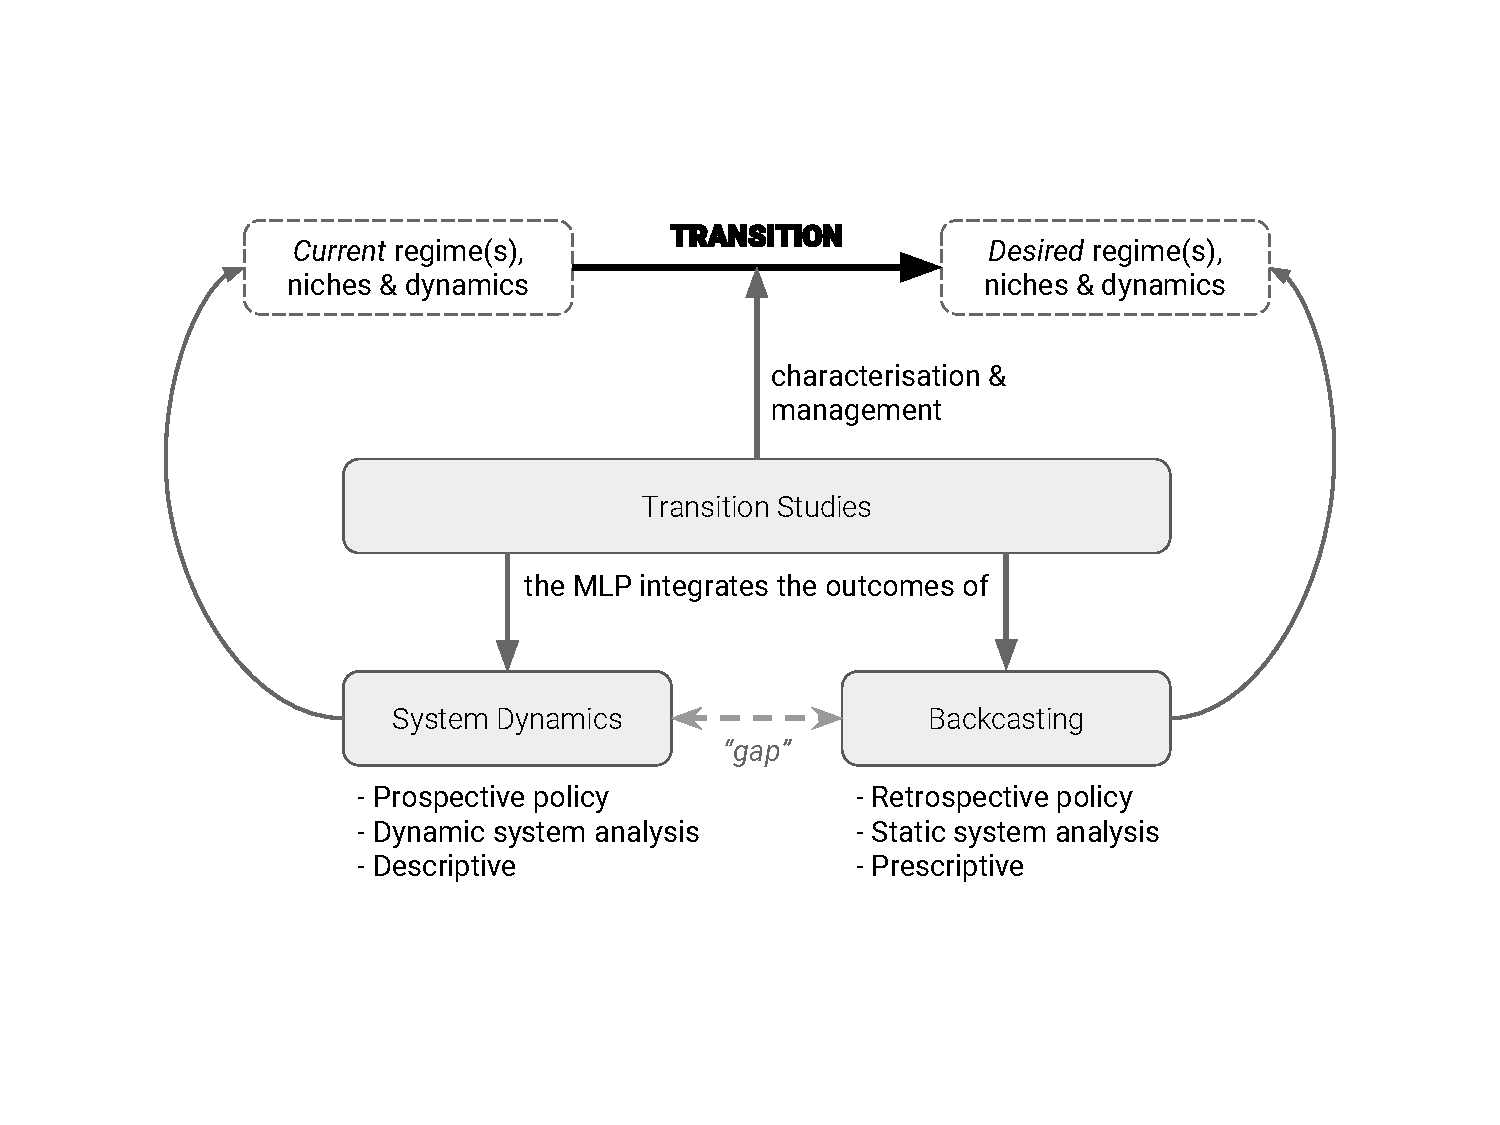
\includegraphics[width=\linewidth]{figures/discussion-methods.pdf}
\caption{Discussion of the methodology and why transition theory can bridge the gap between futures studies and forecasting tools.}
\label{f:discussion-methodology}
\end{figure}

\todoparagraph{In addition to the previous TODO note, the transitions theory reference frame can act as the common narrative that \textcite{creutzig2015_EvolvingNarrativesLow} is looking for in his paper. Discuss this!}

\todoparagraph{Clearly, the CLDs developed are not the ultimate depiction of the automobility system. Even more, they are not indeed the only representation of the very concepts that they model (land-use patterns, cultural legitimacy, PT vs car competence). Rather, they should be seen as an example of the potential that CLDs have for (a) describing system feedback structures and (b) conveying that information in an understandable way for decision makers and (transition) researchers alike. Many other perspectives could have been taken to model the system, at this highly abstract level. The approach taken in this thesis for each of the AUTOLOCK model components is meant to provide enough basis for a discussion of the dynamic behaviour of the automobility system. Furthermore, the focus on abstract concepts and the loose system boundary (e.g., the inclusion of ideological discourses in the culture legitimatory perspective) try to illustrate the difficulty in dealing with such a complex issue. In conclusion, the use of transition theories to put all the insights from the CLD into perspective is the key contribution of the thesis, rather than an accurate and/or indisputable representation of reality.}

\todoparagraph{
-- normative assumptions\\
-- SSP1 vs SSP\{2,3,4,5\} $\rightarrow$ what would happen?\\
-- \textit{realistic} vs \textit{idealistic} approaches: backcasting from a vision cannot pretend to be realistic. This is in clear contrast to the common setting for scientific research, which is based in forecasting methodologies.\\
}

\todoparagraph{
-- lack of ``fuels'' perspective and other technological aspects\\
-- lack of transition-management features (really? or is it done on another level, above the model?)\\
-- lack of other perspectives, due to (a) lack of time and (b) the fact that a ``complete'' model is out of scope and reach for this thesis.
}

\todoparagraph{
-- lack of quantitative figures for both the narrative/backcasting portion of the results and the CLD\\
-- lack of simulation analysis to assess the extent and pace of change in the dynamic feedback structure of the system
}